\chapter{Espacios de Sobolev}

A lo largo de los temas 1 y 2, hemos construido una serie de herramientas básicas en la resolución de ciertos modelos matemáticos. A continuación, vamos a enlazar los conceptos vistos anteriormente y desarrollar los primeros modelos de esta asignatura.

\section{Enlace}

Antes de definir los \textit{espacios de Sobolev}, recordemos algunas propiedades del espacio 
\[L^2(a,b)=\displaystyle\{\funcion{f}{(a,b)}{\R}\;:\; \integral{a}{b}{|f(x)|^2dx<+\infty}\displaystyle\}\]
La norma de este espacio venía dada por $\norm{f}_2=\sqrt{\integral{a}{b}{f(x)^2dx}}$ e inducía el siguiente producto escalar: $<f,g>=\integral{a}{b}{f(x)g(x)dx}$ (nótese que no usamos el conjugado de $g$ ya que estamos trabajando sobre $\R$, no sobre $\C$). Además, $L^2(a,b)\subset L^1(a,b)$ ya que 
\[
\integral{a}{b}{f(x)}=\integral{a}{b}{|f(x)|\cdot 1dx}\leq \left(\integral{a}{b}{f(x)^2dx}\right)^{1/2}\left(b-a\right)^{1/2}
\]
donde hemos usado la desigualdad de Schwartz para el último paso. Con estas propiedades en mente, podemos definir el primer espacio de Sobolev:
\[
\sobolev{1}=\conjunto{f\in\lebesgue{2}: f \text{ tiene derivada débil }f' \text{ y } f'\in\lebesgue{2}}
\]
Este espacio tiene la particularidad de que también cuenta con un producto escalar:
\[
<f,g>=\integral{a}{b}{f(x)g(x)dx}+\integral{a}{b}{f'(x)g'(x)dx}
\]
De es producto se induce la siguiente norma:
\[
\normasobolev{1}{f}=\sqrt{\integral{a}{b}{f(x)g(x)dx}+\integral{a}{b}{f'(x)g'(x)dx}}
\]
Por supuesto, $\sobolev{1}$ es un espacio de Hilbert con la norma $\norm{f}=\sqrt{\norm{f}^2_2+\norm{f'}_2^2}$. Es importante recordar que si $f\in\sobolev{1}$, no tiene por qué ser continua (como muestra \textit{The devil staircase}), pero podemos elegir un representante continuo en su clase de equivalencia, es decir, $\sobolev{1}\hookrightarrow C[a,b]$.
\begin{lemma}
Sea una función $f$, arbitraria, con derivada débil $g$, y denotamos por $\tilde{f}$ a su representante continuo. Entonces:
\[
\forall x,y\in(a,b) \espacio \tilde{f}(y)-\tilde{f}(x)=\integral{x}{y}{g(s)ds}
\]
\end{lemma}
\begin{proof}
Sea $x_0\in(a,b)$. Definimos $\funcion{h}{\R}{\R}$ por 
\[h(x)=\integral{x_0}{x}{g(s)ds} \;\;\forall x\in\R\] 
Por el teorema \ref{fundamentalcalculo}, $h$ es derivable débil con $h'=g$. Luego $h$ y $f$ tienen la misma derivada débil, aplicando la proposición \ref{derivadadebilcero} a $h-f$, tenemos que:
\[
h(x)=f(x)+C \;a.e \;\in(a,b)
\]
para alguna constante $C\in\R$. Cambiando $f$ por su representante continuo:
\[
h(x)=\tilde{f}(x)+C \Rightarrow \tilde{f}(x)=h(x)-C
\]
Repetiendo el mismo razonamiento con $y\in(x,b)$:
\[
h(y)=\tilde{f}(y)+C \Rightarrow \tilde{f}(y)=h(y)-C
\]
Restnado ambas expresiones:
\[
\tilde{f}(y)-\tilde{f}(x)=h(y)-C-h(x)+C=\integral{x_0}{y}{g(s)ds}-\integral{x_0}{x}{g(s)ds}=\integral{x}{y}{g(s)ds}
\]
\end{proof}
\begin{remark}
\label{desigualdadcomun}
Tenemos la siguiente desigualadad (en general):
\[
h\in\lebesgue{2} \Rightarrow \norm{h}_1\leq \norm{h}_2(b-a)^{1/2}
\]
\end{remark}
\begin{prop}\label{inclusion continua}
La aplicación inclusión $\funcion{i}{\sobolev{1}}{C[a,b]}$, definida por $f\mapsto\tilde{f}$ (su representante continuo), es continua.
\end{prop}
\begin{proof}
Tenemos que ver si existe una constante $C\in\R^+$ de forma que
\[
\norm{i(f)}_{\infty}=\norm{\tilde{f}}_\infty\leq C\normasobolev{1}{f}
\]
Tomamos $x,y\in(a,b)$, usando el lema anterior:
\[
\tilde{f}(x)-\tilde{f}(y)=\integral{x}{y}{g(s)ds} \Rightarrow \norm{\tilde{f(x)}}_1\leq\norm{\tilde{f}(y)}_1+\norm{g}_1
\]
Aplicando la desigualdad de la nota \ref{desigualdadcomun}:
\[
\norm{\tilde{f}(x)}_1\leq \norm{\tilde{f}(y)}_1+\norm{g}_2(b-a)^{1/2}
\]
Integrando respecto de $y$:
\[
(b-a)\norm{\tilde{f}(x)}_1\leq \norm{\tilde{f}(y)}_2(b-a)^{1/2}+\norm{g}_2(b-a)^{3/2}
\leq (b-a)\norm{\tilde{f}(x)} \Rightarrow
\]
\[
\norm{\tilde{f}(x)}_1\leq c_1\norm{f}_2+c_2\norm{g}_2 \Rightarrow
\]
\[
\norm{\tilde{f}}_\infty\leq c_1\norm{f}_2+c_2\norm{g}_2 \leq (c_1+c_2)\normasobolev{1}{f}
\]
\textbf{REVISAR ESTA DEMOSTACION}
\end{proof}
Además, si $f\in C^1[a,b]$, tiene derivada clásica, luego también tiene derivada débil, luego $f\in\sobolev{1}$. Resumiendo, hemos construido la siguiente cadena:
\[
C^1[a,b]\subset\sobolev{^1}\subset C[a,b]\subset \lebesgue{2}
\]
Definimos ahora el siguiente espacio de Sobolev:
\[
\sobolev{2}=\conjunto{f\in\lebesgue{2}: \exists f',f''\in\lebesgue{2}\text{ (débiles)}}
\]
Usando la propiedad \ref{derivadanesima}, tenemos que $\sobolev{2}\subset C^1[a,b]$ y repitiendo el argumento anterior $C^2[a,b]\subset \sobolev{2}$, es decir:
\[
C^2[a,b]\subset \sobolev{2}\subset C^1[a,b]
\]
Repitiendo este proceso iterativamente, podemos definir el $n$-ésimo espacio de Sobolev:
\[
\sobolev{n}=\conjunto{f\in\lebesgue{2}: \exists f',\dots,f^{n)}\in\lebesgue{2} \text{ (débiles)}}
\]
con la propiedad:
\[
C^{n}[a,b]\subset\sobolev{n}\subset C^{n-1}[a,b]\subset\sobolev{n-1}\subset\dots\subset\sobolev{1}\subset\lebesgue{2}
\]

¿Qué tienen de particular estos espacios? Que son de Hilbert, es decir, vamos a poder usar todas las herramientes que tenemos de Análisis Funcional para resolver algunos problemas como veremos en los siguientes apartados.

\begin{definition}
Diremos que $\funcion{F}{[a,b]\times\R^2}{\R}$ es una \textit{función de Carathéodory} si cumple:
\begin{enumerate}[(a)]
\item Para casi todo punto $x\in(a,b)$, $F(x,y,p)$ es continua en $(y,p)$.
\item Para casi todo punto $(y,p)\in\R^2$, la función $x\mapsto F(x,y,p)$ es medible.
\item Dado $K\subset[a,b]\times\R^2$ compacto, existe una función $m_k(x)\in\lebesgue{1}$ tal que $\valorabsoluto{F(x,y,p)}\leq m_k(x)$ $\forall(x,y,p)\in K$.
\end{enumerate}
\end{definition}

Para que la teoría que vamos a desarrollar a continuación tenga sentido, vamos a imponer de ahora en adelante que $F$, $F_y$ y $F_p$ sean de Carathéodory. Haciendo uso de la propiedad (c), podemos definir el funcional $\funcion{L}{\sobolev{1}}{\R}$:
\[
L(y)=\integral{a}{b}{F(x,y(x),y'(x))dx}
\]
que está bien definido ya que que $F$ es medible y está acotada por una función que es integrable. Tomando $\phi\in\soportecompacto$, podemos definir otra función $\funcion{g}{[a,b]}{\R}$ por $g(s)=L(y+s\phi)$, derivarla respecto a $s$ y evaluarla en 0 (a esta expresión la llamamos \textit{derivada de y a lo largo de $\phi$}):
\[
g'(0)=DL_y(\phi)=\integral{a}{b}{F_y(x,y(x),y'(x)dx}+\integral{a}{b}{F_p(x,y(x),y'(x)dx}
\]
\newpage

\section{Modelos de cuerdas y puentes}

Procedemos a la introducción del \textit{modelo de cuerdas}. Comenzaremos realizando el planteamiento más simple, densidad constante y extremos fijos. Posteriormente, eliminaremos la primera hipótesis y resolveremos dos casos: en el primero partimos de una función de densidad dada explícitamente. Por el contrario, en el segundo caso, lo resolveremos dada una función de densidad arbitraria. A continuación, supondremos que el puente se haya \textit{sujeto} por varias cuerdas elásticas. Finalmente, no supondremos fijos los extremos.

Aunque ya hemos desarrollado una cantidad de resultados considerable, todavía precisamos de ciertos resultados, mayoritariamente del \textit{Análisis Funcional}, que iremos introduciendo al mismo tiempo que el modelo. Como estamos trabajando sobre espacios de Sobolev, que son de Hilbert, podremos usarlos sin mucha complicación.

\begin{figure}[h]
   \center
  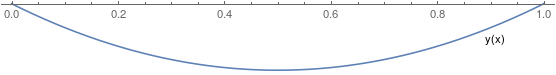
\includegraphics[scale=0.5]{img/cuerdanormal.png}
\end{figure}

\subsection{Extremos fijos y densidad constante}

Supongamos tener una \textit{cuerda elástica}, colgada entre dos puntos, 0 y 1, es decir, nuestra cuerda está representada por una función $\funcion{y}{[0,1]}{\R}$ en $\sobolev{1}$ tal que $y(0)=y(1)=1$. El objetivo del modelo será encontrar la \textit{cuerda} de mínima energía. En este caso, vamos a suponer que la \textit{densidad} de la cuerda es una constante $m\in\R^+$. 

Denotamos por $E_p$ a la energía potencial y por $E_e$ a la energía elástica:
\[
E_e=\frac{1}{2}\integral{0}{1}{y'(x)^2dx} \espacio\espacio E_p=\integral{0}{1}{my(x)dx}
\]
Minimizar la energía total de la cuerda, es lo mismo que minimizar el funcional:
\[
L(y)=\frac{1}{2}\integral{0}{1}{y'(x)^2dx}+\integral{0}{1}{my(x)dx}
\]
Usando la notación usual:
\[
L(y)=\integral{0}{1}{F(x,y,p)dx} \; \text{ donde } \;\; F(x,y,p)=\frac{1}{2}p^2+my
\]
Supongamos que $y\in\sobolev{1}$ es un punto crítico del funcional $L:\sobolev{1}\longrightarrow\R$ para poder usar la teoría de la \textit{ecuación de Euler}.
Si calculamos las derivadas parciales de $F(x,y,p)$:
\[
Z(x)=F_p(x,y,p)=p=y'(x) \espacio Z'(x)=F_y(x,y,p)=m
\]
vemos que $Z(x)$ tiene derivada débil ($Z'(x)$), como consecuencia, $y'(x)$ es continua (proposición \ref{representantecontinuo}). Pero además, $Z'(x)=(y'(x))'=y''(x)=m$, continua, por lo tanto $y\in C^2[0,1]$. En resumen, tenemos que resolver la siguiente EDO de segundo orden:
\[
\left\{
\begin{array}{rl}
y''(x) & = m \\
y(0) & = 0 \\
y(1) & = 0
\end{array}
\right.
\]
Si recordamos algo de ecuaciones diferenciales, nos damos cuenta de que las condiciones iniciales están \textit{mal planteadas}. Para poder resolver la ecuación, necesitamos dos conciones sobre el mismo punto: una en $y$ y otra en $y'$. Lo podemos solucionar usando el llamado \textit{método de tiro}, que consiste en darle un valor arbitrario a la condición que nos falta, resolver la ecuación y despejar el valor posteriormente. Asumiendo que $y'(0)=\alpha\in\R$, nos queda:
\[
\left\{
\begin{array}{rl}
y''(x) & = m \\
y'(0) & = \alpha \\
y(0) & = 0
\end{array}
\right.
\]
con solución $y(x)=\integral{0}{x}{\left(\alpha+msds\right)}=m\frac{x^2}{2}+\alpha x$. Usando $y(1)=0$, obtenemos que $\alpha=-\frac{m}{2}$. Por lo que la solución del modelo es:
\[
y(x)=\frac{m}{2}x(x-1) \;\; \forall x \in[0,1]
\] 

\subsection{Extremos fijos y densidad no constante}

El planteamiento es igual al anterior, pero suponemos que la densidad en lugar de ser constante es la función $\funcion{q}{[0,1]}{\R}$ dada por:
\[
q(x)=\left\{\begin{array}{cc}
1 & x \in[0,\frac{1}{2}] \\
\frac{1}{2} & x \in(\frac{1}{2}, 1] 
\end{array}
\right.
\]
Cabe resaltar que $q(x)$ no es continua (presenta un salto en $x=\frac{1}{2}$, pero no importa a la hora de resolverlo. En este caso, el funcional viene dado por:
\[
L(y)=\integral{0}{1}{\frac{1}{2}y'(x)^2+q(x)y(x)dx}
\]
con $F(x,y,p)=\frac{1}{2}p^2+q(x)y$, $F_p(x,y,p)=p$, $F_y(x,y,p)=q(x)$. La ecuación diferencial a resolver es (usando de nuevo el método de tiro):
\[
\left\{
\begin{array}{rl}
y''(x) & = q(x) \\
y(0)  = 0,y'(0) & = \alpha \\
y(1)= 0, y'(1) & = \beta
\end{array}
\right.
\]
Tenemos el problema de que $y\notin C^2[0,1]$. Intentemos arreglarlo:
\begin{itemize}
\item Si $x\in(0,\frac{1}{2}) \Rightarrow y''(x)=1 \Rightarrow y\in C^2(0,\frac{1}{2}) \Rightarrow y'(x)=\integral{0}{x}{1dx}+y'(0)=x+\alpha$\\
 $\Rightarrow y(x)=\integral{0}{x}{x+\alpha dx}=\frac{x^2}{2}+x\alpha$.
\item Si $x\in(\frac{1}{2},1) \Rightarrow y''(x)=1/2 \Rightarrow y\in C^2(\frac{1}{2},1) \Rightarrow y'(x)=y'(1)-\integral{x}{1}{\frac{1}{2}dx}=\beta+\frac{x}{2}-\frac{1}{2}$\\
$\Rightarrow y(1)-y(x)=\integral{x}{1}{\frac{x}{2}-\frac{1}{2}+\beta dx}\Rightarrow y(x)=-\frac{x^2}{2}+\frac{x}{2}+\beta(x-1)$
\end{itemize}
Quedando:
\begin{equation}\label{y}
y(x)=\left\{
\begin{array}{cc}
\frac{x^2}{2}+x\alpha & x\in[0,1/2) \\
-\frac{x^2}{2}+\frac{x}{2}+\beta(x-1) & x\in(1/2,1]
\end{array}
\right.
\end{equation}

\begin{equation}\label{yprima}
y'(x)=\left\{
\begin{array}{cc}
x+\alpha & x\in[0,1/2) \\
-x+\frac{1}{2}+\beta & x\in(1/2,1]
\end{array}
\right.
\end{equation}

Ahora tenemos que resolver el sistema de $\alpha$ y $\beta$. Obtendremos dos ecuaciones de imponer que $y$ e $y'$ sean continuas en $\frac{1}{2}$, es decir, de que las dos partes evaluadas en ese punto coincidan. Por lo que a partir de \eqref{y} y \eqref{yprima} conseguimos,evaluando en $\frac{1}{2}$ e igualando:
\begin{equation}
\left\{
\begin{array}{cc}
\alpha+\beta & =0 \\
\alpha-\beta & =-\frac{1}{2}
\end{array}
\right.
\end{equation}
Resolviendo el sistema, $\alpha=-1/4$, $\beta=1/4$. Quedando finalmente la siguiente solución al modelo:
\begin{equation}\label{y}
y(x)=\left\{
\begin{array}{cc}
\frac{x^2}{2}-\frac{x}{4} & x\in[0,1/2) \\
\frac{-x^2}{2}+\frac{x}{2}+\frac{1}{4}(x-1) & x\in(1/2,1]
\end{array}
\right.
\end{equation}

\begin{figure}[h]
   \center
  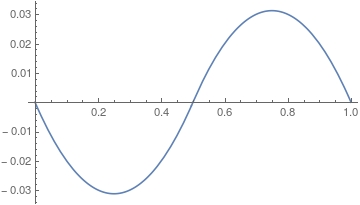
\includegraphics[scale=0.6]{img/puenteflotante.png}
\end{figure}

\textbf{el puente sigue flotanto x'dddddddddds}

\subsection{Extremos fijos y densidad arbitraria}

El planteamiento es igual al caso más simple, pero ahora la función de densidad, $q(x)$, la consideraremos en $\lebesgue{\infty}$. Sin la expresión de la función $q(x)$, no podemos resolver el problema de forma explícita, pero sí podemos asegurar la existencia de solución. El siguiente procedimiento lo repetiremos varias veces: definimos un espacio en donde buscaremos nuestra solución ($\sobolevcero{1}$), plantearemos el problema (condición de extremal), definiremos un producto escalar y demostraremos que el espacio definido con ese producto escalar es de Hilbert, para usar el Teorema de Riesz-Fréchet.

\begin{remark}
El espacio $\lebesgue{\infty}$ se definía como:
\[
\lebesgue{\infty}=\{\funcion{f}{(a,b)}{\R}|f\text{ medible y esencialmente acotada}\}
\]
con la norma:
\[
\norm{f}_\infty = \suppess_{x\in(a,b)\;a.e}|f(x)|
\]
\end{remark}

Comencemos definiendo nuestro espacio de soluciones:
\[
\sobolevcero[a,b]{1}=\conjunto{y\in\sobolev{1}: y(a)=y(b)=0}
\]
Recordemos que en este espacio están las funciones de $\lebesgue{2}$, que tienen derivada débil. Por lo tanto, por la proposición \ref{representantecontinuo} podemos elegir una $y$ que sea continua.
\begin{prop}
El espacio vectorial $\sobolevcero{1}$, es cerrado.
\end{prop}   
\begin{proof}
Sea una secuencia de funciones convergentes en $\sobolevcero{1}$, $f_n\longrightarrow f$. Usando la proposición \ref{inclusion continua} y $\sobolevcero{1}\subset C^{1}[a,b]$, tenemos que $f_n(a)\longrightarrow f(a)$ y $f_n(b)\longrightarrow f(b)$. Luego $f_n(a)=f_n(b)=0 \;\forall n\in\N \Rightarrow f(a)=f(b)=0 \Rightarrow f\in\sobolevcero{1}$.\\
\end{proof}

Una vez definido nuestro nuevo espacio, pasamos a resolver el modelo. Como de costumbre, suponemos que $y\in\sobolevcero[0,1]{1}$ es extremal y usamos la teoría de Euler:
\[
L(y)=\frac{1}{2}\integral{0}{1}{y'(x)^2dx}+\integral{0}{1}{q(x)y(x)dx}
\]
Usando la notación usual:
\[
L(y)=\integral{0}{1}{F(x,y,p)dx} \; \text{ donde } \;\; F(x,y,p)=\frac{1}{2}p^2+q(x)y
\]
Calculando sus derivadas parciales
\[
F_p(x,y,p)=p \espacio F_y(x,y,p)=q(x)
\]
podemos calcular $\funcion{DL_y}{\sobolevcero[0,1]{1}}{\R}$ y usar la concidición de extremal de $y$ (teorema \ref{theorem:1.7}):
\[
DL_y(\phi)=\integral{0}{1}{y'(x)\phi'(x)dx}+\integral{0}{1}{q(x)\phi(x)dx}=0 \espacio \forall \phi\in\sobolevcero[0,1]{1}
\]
Si lo miramos como una derivada débil, vemos que si $Z(x)=y'(x) \Rightarrow Z'(x)=q(x) \Rightarrow y''(x)=q(x)$, en sentido débil.
\begin{definition}
\label{soluciondebil}
$y\in\sobolevcero{1}$ es \textit{solución débil} de $y''(x)=q(x) \; \forall x 
\in [a,b]$, si se verifica:
\[
\integral{0}{1}{y'(x)\phi'(x)dx}+\integral{0}{1}{q(x)\phi(x)dx}=0 \espacio \forall \phi\in\sobolevcero[0,1]{1}
\]
\end{definition}
Cabe resaltar, el hecho de que en la anterior definición, $y$ está en $\sobolevcero[0,1]{1}$ y estamos resolviendo una EDO de segundo orden, es decir, no sabemos nada sobre la segunda derivada de $y$ (solo de la primera).

Definimos un producto escalar en $\sobolevcero[a,b]{1}$ y veamos que es de Hilbert:
\begin{prop}
El espacio $\sobolevcero[a,b]{1}$ con el siguiente producto escalar:
\[
f,g\in\sobolevcero[a,b]{1}, \espacio <f,g>=\integral{a}{b}{f'(x)g'(x)dx}
\]
es un espacio de Hilbert.
\end{prop}
\begin{proof}
Sea $f_n\in\sobolevcero{1} \;\forall n\in\N$ una sucesión de Cauchy, entonces:
\[
\forall \varepsilon>0 \; \exists n_0: \; n,m\geq n_0 \; \normasobolevcero{1}{f_n-f_m}<\varepsilon
\]
Recordemos que si tenemos un producto escalar definido, podemos expresar la norma de un elemento del espaico como la raíz cuadrada del producto escalar de el elemento consigo mismo, es decir:
\[
\normasobolevcero{1}{f}=\sqrt{<f,f>}
\]
Usando esa propiedad:
\[
\varepsilon > \normasobolevcero{1}{f_n-f_m}=\sqrt{<f_n-f_m,f_n-f_m>}=\sqrt{\integral{a}{b}{(f_n(x)-f_m(x))^2dx}}=\norm{f_n'-f_m'}_2
\]

Luego $f_n'$ converge a una cierta $g$ en $\lebesgue{2}$. Dado que $\tilde{f_n}(a)=0$, se obtiene que
\[
\tilde{f_n}(x)=\integral{a}{x}{f'_n(s)ds}\longrightarrow\integral{a}{x}{g(s)ds}
\]
Luego tomo
\[
f(x)=\integral{a}{x}{g(s)ds}=\limitemasinfinito{n}{\tilde{f_n}(x)}, \;\; x \in[a,b]
\]
Ya tenemos candidato a límite. Veamos que $f\in\sobolevcero{1}$. En principio:
\[
f(b)=\integral{a}{b}{g(s)ds}=\limitemasinfinito{n}{f'_n(s)ds}=\tilde{f_n}(b)-\tilde{f_n}(a)=0
\]
Además, $f$ tiene derivada débil (igual a $g$) por el teorema \ref{fundamentalcalculo}.
\end{proof}

Una vez comprobado que el espacio es de Hilbert, solo nos falta recordar el Teorema de Riesz-Fréchet:
\begin{theorem}[Riesz-Fréchet]
\label{riesz-frechet}
Si $H$ es un espacio de Hilbert y $f\in H^*$, existe $y\in H$ tal que:
\[
f(x)=<x,y> \; \forall x\in H
\]
\end{theorem}

Sea ahora $\phi\in\sobolevcero{1}$, definimos $\funcion{R}{\sobolevcero{1}}{\R}$ por $R(\phi)=-\integral{a}{b}{q(x)\phi(x)dx}\in\left(\sobolevcero{1}\right)^*$. Por el teorema de Riesz-Fréchet, existe $y\in\sobolevcero{1}$ tal que $R(\phi)=<y,\phi>$.

Si desarrollamos la última expresión, nos damos cuenta de que es igual a la condición en la definición \ref{soluciondebil}, que es justo lo que buscábamos.

\subsection{Puente sujeto por cuerdas}

Al modelo del puente anterior le vamos a añadir unas cuerdas elásticas para soportarlo, cada una con una constante de elasticidad distinta, dado por $K(x)\geq 0$.
Si $K(x)=0$ en algún punto $x\in[0,1]$, significa que en ese punto no hay cuerda sujetando a la de abajo.
\begin{figure}[H]
   \center
  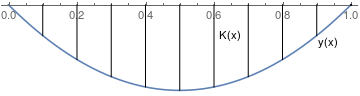
\includegraphics[scale=0.6]{img/puentecuerdas.png}
\end{figure}
En esta nueva versión del modelo tenemos que tener en cuentra otra energía más, la aportada por los cables, $E_c$:
\[
E_c=\frac{1}{2}\integral{0}{1}{K(x)y^2(x)dx}
\]
Con lo que el funcional quedaría:
\[
L(y)=\frac{1}{2}\integral{0}{1}{y'(x)^2dx}+\frac{1}{2}\integral{0}{1}{K(x)y(x)^2dx}+\integral{0}{1}{q(x)y(x)dx}
\]
Usando la notación usual:
\begin{equation}\label{funcionalpuente}
L(y)=\integral{0}{1}{F(x,y,p)dx} \; \text{ donde } \;\; F(x,y,p)=\frac{1}{2}p^2+\frac{1}{2}K(x)y^2+q(x)y
\end{equation}
Suponiendo que $y\in\sobolevcero[0,1]{1}$ es extremal, la condición de punto crítico es:
\[
DL_y(\phi)=\integral{0}{1}{y'(x)\phi'(x)dx}+\integral{0}{1}{\left(K(x)y(x)+q(x)\right)\phi(x)dx}=0 \;\; \forall \phi\in\sobolevcero[0,1]{1}
\]
Denotando $Z(x)=y'(x)$ y viendo la expresión anterior en sentido débil, tenemos que $Z'(x)=K(x)y(x)+q(x)$ es su derivada débil. Luego la EDO de orden 2 de este modelo es (que la obtenemos a partir de la ecuación de Euler):
\[
-y''(x)=+K(x)y(x)+q(x)=0
\]
Ahora, al igual que en el modelo anterior, vamos a definir un cierto producto escalar de forma que el teorema de Riesz-Frechét nos de la existencia de solución. Pero antes, vamos a desarrollar la teoría necesaria para demostrarlo:

\begin{remark}
\begin{itemize}
\label{notafuncional}
\item Dos normas, $||\cdot||_1$ y $||\cdot||_2$, se dicen comparables si existe $c_1\in\R^+$ tal que $\norm{x}_1\leq c_1\norm{x}_2$.
\item Si además existe otra constante $c_2\in\R^+$ tal que$\norm{x}_2\leq c_2\norm{x}_1$, entonces se dicen equivalentes.
\item (Tª Isomorfismos de Banach) Si $\funcion{f}{B}{B'}$ es una aplicación lineal, continua y biyectiva entre dos espacios de Banach, $B$ y $B'$, entonces $F^{-1}$ es continua.
\end{itemize}

Como corolario de ese teorema tenemos que si en un espacio de Banach, $B$, existen dos normas comparables, entonces las normas son equivalentes. Este resultado se obtiene fácilmente al aplicar el teorema anterior con $f=Id_B$.
\end{remark}

\begin{prop}[Lema de Poincaré]
\label{lemapoincare}
Existe $\lambda\in\R^+$ constante tal que se verifica
\[
\integral{a}{b}{f(x)^2dx}=\lambda\integral{a}{b}{f'(x)^2dx} \espacio \forall f\in\sobolevcero{1}
\]
\end{prop}

\begin{proof}

En $\sobolevcero{1}$ tenemos dos normas:
\[
\normasobolevcero{1}{f} = \sqrt{\integral{a}{b}{f'(x)^2dx}}, \espacio \normasobolev{1}{f}=\sqrt{\integral{a}{b}{f(x)^2dx}+\integral{a}{b}{f'(x)^2dx}}
\]

Evidentemente la desigualdad que necesitamos para que sean comparables se cumple: $\normasobolevcero{1}{f}\leq \normasobolev{1}{f}$. Luego existe $C\in\R$ tal que $\normasobolev{1}{f}\leq C\normasobolevcero{1}{f}$, es decir:
\[
\integral{a}{b}{f(x)^2dx}+\integral{a}{b}{f'(x)^2dx}\leq C^2\integral{a}{b}{f'(x)^2dx}
\]
Por tanto:
\[
\integral{a}{b}{f(x)^2dx}\leq (C^2-1)\integral{a}{b}{f'(x)^2dx}
\]

\end{proof}

\begin{prop}
El espacio $\sobolevcero[a,b]{1}$ con el siguiente producto escalar:
\[
f,g\in\sobolevcero[a,b]{1}, \espacio <f,g>=\integral{a}{b}{f'(x)g'(x)dx}+\integral{a}{b}{K(x)f(x)g(x)dx}
\]
con $K\in\lebesgue{2}$, $K(x)\geq 0$ $\forall x\in[a,b]$, es un espacio de Hilbert.
\end{prop}
\begin{proof}
Usando el lema \ref{lemapoincare}, es fácil ver que $\normasobolevcero{1}{\cdot}$ y $\normasobolev{1}{\cdot}$ son comparables, luego equivalentes por la nota \ref{notafuncional}. Como ya vimos al principio del tema, la norma $\normasobolev{1}{\cdot}$ es completa, luego $\normasobolevcero{1}{\cdot}$ también lo es, por ser ambas equivalentes.
\end{proof}

Usando ese producto escalar, la expresión \eqref{funcionalpuente} se puede reescribir como:

\[
L(y)=\frac{1}{2}<y,y>+R(y)
\]

donde $R(y)=\integral{a}{b}{q(x)y(x)dx}$ e $y\in\sobolevcero{1}$, y por el teorema de representación de Riesz existe punto crítico.

\subsection{Teorema de Lax-Milgran}

Para dejar el puente libre, primero necesitamos ver nuestro funcional $L$ desde otro punto de vista. Para ello, vamos a ver una serie de definiciones y propiedades abstractas sobre los \textit{funcionales cuadráticos}, lo que nos va a permitir enunciar el teorema de Lax-Milgran, que nos dará la existencia de solución en esta última versión del modelo.

\begin{definition}\label{formabilineal}
Dados un cuerpo $K$ y un $K-$espacio vectorial $V$, una forma bilineal es una aplicación $\funcion{f}{V\times V}{K}$ que verifica:
\begin{enumerate}[(a)]
\item $f(u_1+u_2,v)=f(u_1,v)+f(u_2,v)$
\item $f(u, v_1+v_2)=f(u,v_1)+f(u,v_2)$
\item $f(au,v)=af(u,v)$
\item $f(u,av)=af(u,v)$
\end{enumerate}
para cualquier $a\in K$ y $u,v,u_1,u_2,v_1,v_2\in V$.

Una propiedad que necesitaremos es:
\[
f\left(\sum_ia_iu_i,\sum_jb_jv_h\right)=\sum_i\sum_ja_ib_jf(u_i,v_j)
\]

\end{definition}

\begin{definition}
Una forma bilineal $\funcion{f}{V\times V}{K}$ se dice simétrice si verifica:
\[
f(u,v)=f(v,u) \espacio \forall u,v\in V
\]
\end{definition}

\begin{definition}
Sea $H$ un espacio de Hilbert arbitrario, $\funcion{A}{H\times H}{\R}$ una forma bilineal, continua y simétrica y $\funcion{R}{H}{\R}$ una aplicación lineal y continua. Llamamos funcional cuadrático a la aplicación $\funcion{L}{H}{\R}$ dada por
\[
L(y)=\frac{1}{2}A(y,y)-R(y) \espacio\forall y\in H
\]
\end{definition}

\begin{definition}
Sea $\funcion{L}{H}{\R}$ una forma cuadrática. Diremos que es coerciva si existe una constante $\alpha\in\R^+$ tal que:
\[
A(u,u)\geq \alpha\norm{u}^2 \espacio \forall u\in H
\]
\end{definition}

\begin{prop}
Sea un espacio de Hilbert $H$ y $\funcion{L}{H}{\R}$ una forma cuadrátrica en ese espacio.
Entonces, la aplicación $\funcion{\norm{\cdot}_H}{H}{\R^+_0}$ definida por 
\[
\norm{u}_H=\sqrt{A(u,u)} \espacio \forall u\in H
\]
donde $\funcion{A}{H\times H}{\R}$ es la forma bilineal asociada a $L$, es una norma, y es equivalente a la norma natural de $H$.
\end{prop}
\begin{proof}
El hecho de que $\norm{\cdot}_H$ es una norma es sencillo de comprobar ya que $A$ define un producto escalar en $H$.

Sea $\funcion{\norm{\cdot}}{H}{\R}$ la norma de $H$. Necesitamos encontrar dos constante $c_1,c_2\in\R^+$ tal que 
\[
c_1\norm{u}\leq \norm{u}_H \leq c_2\norm{u}
\]
La constante $c_2$ la obtenemos por continuidad de la norma $\norm{\cdot}_H$ y la constante $c_1$ de la coercividad de $L$.

\end{proof}

A partir de ahora consideramos $\norm{\cdot}_H$ como nuestra norma por defecto en $H$.

\begin{prop}
Todo funcional cuadrático está acotado inferiormente.
\end{prop}
\begin{proof}
Sea $\funcion{L}{H}{\R}$ un funcional cuadrático, donde $\funcion{A}{H\times H}{\R}$ es su forma bilineal, continua y simétrica y $\funcion{R}{H}{\R}$ es su aplicación lineal y continua.
Vamos a ver que podemos acotar inferiormente la expresión de $L(y)$, con $y\in H$, por una función parabólica hacia arriba.

Como $R$ es continua, entonces $\norm{R(y)}\leq \norm{R}\norm{y} \Rightarrow -\norm{R(y)} \geq -\norm{R}\norm{y}$. Además, como $L$ es coerciva, existe cierta constante $C\in\R^+$ tal que $A(y,y)\geq C\norm{y}^2$. Combinando esas dos acotaciones, obtenemos:
\[
L(y)=\frac{1}{2}A(y,y)-R(y)\geq \frac{1}{2}C\norm{y}^2-\norm{R}\norm{y}
\]
Para ver con más claridad la parábola, hacemos el cambio $s=\norm{y}$, obteniendo una nueva función $P$ dependiente de las dos constantes $C$ y $\norm{R}$: $P(s)=\frac{1}{2}s^2-s\norm{R}$. Derivando e igualando a 0, obtenemos fácilmente que el mínimo de la parábola $P$ se alcanza en $s=\frac{\norm{R}}{C}$. Luego:
\[
L(y)\geq \frac{\norm{R}}{C} \espacio \forall y\in H 
\]

\end{proof}

\begin{theorem}[Lax-Milgran]
\label{laxmilgran}
Sea $\funcion{L}{H}{\R}$ un funcional cuadrático. Si $L$ es coercivo, entonces tiene mínimo absoluto en $H$.
\end{theorem}

\begin{prop}[condición de punto crítico]
\label{puntocritico}
Sea $\funcion{L}{H}{\R}$ un funcional cuadrático coercivo, $y\in H$, $\phi\in\soportecompacto$. Entonces existe $y\in H$ verificando:
\[
A(\phi,y)-R(\phi)=0 \espacio \forall\phi\in\soportecompacto
\]

Además, el punto $y$ es el mínimo de $L$.
\end{prop}
\begin{proof}
Calculemos primero la expresión explícita de $g(s)$:
\[
g(s)=L(y+s\phi)=\frac{1}{2}A(y+s\phi,y+s\phi)-R(y+s\phi)
\]
Desarrollamos el primer término (usando la última propiedad en la definición \ref{formabilineal}):
\[
A(y+s\phi,y+s\phi)=A(y,y)+sA(y,\phi)+sA(\phi,y)+s^2A(\phi,\phi)=s^2A(\phi,\phi)+2sA(\phi,\phi)+A(y,y)
\]
Para el segundo término, usamos que $R$ es lineal:
\[
R(y+s\phi)=R(y)+sR(\phi)
\]
Quedándo:
\[
g(s)=\frac{1}{2}\left(s^2A(\phi,y)+2sA(\phi,\phi)+A(y,y)\right)-R(y)-sR(\phi)
\]
Derivando respecto de $s$:
\[
g(s)=sA(\phi,\phi)+A(\phi,y)-R(\phi) \Rightarrow g'(0)=A(\phi,y)-R(\phi)
\]
Luego nuestra condición de punto crítico es:
\[
A(\phi,y)-R(\phi)=0 \espacio \forall\phi\in\soportecompacto
\]

Para le existencia, simplemente tenemos que definir un producto escalar y usar el teorema de Riesz, como en los ejemplos anteriores. Sea $<<u,v>>=A(u,v)$ un producto escalar en $H$, por el teorema \ref{riesz-frechet}, existe $y\in H$ verificando:
\[
<<y,\phi>>=R(\phi) \espacio \forall \phi\in\soportecompacto
\]

Para ver que es mínimo, tomamos $\funcion{g}{\R}{\R}$ definida por $g(s)=L(y+s(z-y))$. Notemos que $y+s(z-y)$ es la recta que una a $z$ con $y$. Tenemos que ver
\[
L(z)>L(y) \espacio \forall z\in H
\]
Que si nos fijamos, es equivalente a ver que
\[
g(1)>g(0)
\]
Que ya lo tenemos porque $s=0$ era el punto mínimo de la parábola.
\end{proof}

Una vez planteada toda la teoría necesaria, podemos volver a nuestro modelo del puente. Recordemos que nuestro funcional  $\funcion{L}{\sobolev{1}}{\R}$ venía dado por la expresión:
\[
L(y)=\frac{1}{2}\integral{a}{b}{y'(x)^2dx}+\frac{1}{2}\integral{a}{b}{K(x)y(x)^2dx}+\integral{a}{b}{q(x)y(x)dx}
\]
donde $q,K\in\lebesgue{\infty}$ y $K(x)\geq k_0 >0\casipordoquier$. La última condición la imponemos porque al dejar los extramos sueltos (lo hemos hecho al considerar como dominio de $L$ el espacio $\sobolev{1}$ en lugar de $\sobolevcero{1}$) necesitemos que el puente siga enganchado por las cuerdas.

Para poder usar la teoría desarrollada anteriormente, necesitamos ver que nuestro funcional es cuadrático. Definimos nuestra forma bilineal, continua y simétrica, y nuestra aplicación lineal y continua:
\[
A(u,v)=\integral{a}{b}{u'(x)v'(x)dx}+\integral{a}{b}{K(x)u(x)v(x)dx}, \; \espacio R(u)=-\integral{a}{b}{q(x)u(x)dx} \;\;\forall u,v\in\sobolev{1}
\]
Pero también necesitamos que $L$ sea coerciva. Usando la hipótesis sobre $K(x)$ es fácil de ver:


\[
A(u,u)=\integral{a}{b}{u'(x)^2dx}+\integral{a}{b}{K(x)u(x)^2dx}\geq\normasobolev{1}{u}^2+k_0\normasobolev{1}{u}^2\geq(1+k_0)\normasobolev{1}{u}^2
\]

Por lo tanto, sabemos que existe mínimo en $\sobolev{1}$. Además de saber que existe, queremos saber algo más sobre su expresión. Como hemos visto antes, los puntos críticos están caracterizados por la expresión:

\[
y\in\sobolev{1} \text{ punto critico } \Leftrightarrow A(y,\phi)=R(\phi) \espacio \forall \phi\in\sobolev{1}
\]
es decir,
\[
\integral{a}{b}{y'(x)\phi'(x)dx}+\integral{a}{b}{K(x)y(x)\phi(x)dx}=-\integral{a}{b}{q(x)\phi(x)dx} \espacio  \forall\phi\in\sobolev{1}
\]
Si en lugar de considerar $\phi$ en $\sobolev{1}$, la consideramos en $\soportecompacto$. Vemos que llamando $z=y'$ y agrupando los términos que tienen $\phi$, llegamos a:
\[
\integral{a}{b}{z(x)\phi'(x)dx}=-\integral{a}{b}{(K(x)y(x)+q(x))\phi(x)dx} \espacio  \forall\phi\in\sobolev{1}
\]

lo que significa que la derivada débil de $z$ es justamente $ky+q$. En particular z está en $\sobolev{1}$, porque todas las funciones que aparecen están en $\lebesgue{2}$. Luego debemos resolver la siguiente ecuación diferencial de orden 2 en $y$:
\[
y''(x)=K(x)y(x)+q(x) \espacio \forall x \in[a,b]
\]
Si imaginamos que $K$ y $q$ son continuas, esa ecuación tendría un gran número de soluciones. De hecho, el conjunto de soluciones sería un espacio biparamétrico (porque la solución depende de las condiciones iniciales sobre $y$ e $y'$). Tenemos que intentar limitarlas de alguna forma.

\begin{prop}
Sea $y\in\sobolev{1}$ (el representante continuo) y $\phi\in\mathcal{D}(\R)$, entonces $y\phi\in\sobolev{1}$.
\end{prop}
\begin{proof}
Para ver que $y\phi\in\sobolev{1}$, necesitamos encontrar su derivada débil. ¿Cuál es nuestro candidato a derivada débil? La derivada clásica, es decir, $z=y'\phi+y\phi'$. Para comprobarlo, tenemos que ver que para toda $\psi\in\soportecompacto$ se tiene:

\[
\integral{a}{b}{(y'(x)\phi(x)+y(x)\phi'(x))\psi(x)dx}+\integral{a}{b}{y(x)\phi(x)\psi'(x)dx}=0
\]
Reordenando los términos que tienen $y$ e $y'$, obtenemos:
\[
\integral{a}{b}{[\phi(x)\psi'(x)+\phi'(x)\psi(x)]y(x)dx}+\integral{a}{b}{[\phi(x)\psi(x)]y'(x)dx}=0
\]
Se cumple que si
$\phi \in \mathcal{D}(\mathbb{R}), \psi \in \mathcal{D}((a,b))$
entonce $\phi\psi \in \mathcal{D}((a,b))$ y
\[
  (\phi\psi)' = \phi'\psi + \phi\psi'
\]
Ahora por ser $y \in \mathcal{H}^1(a,b)$ y
$\hat\phi \in \mathcal{\mathbb{R}}$ tenemos que se cumple
\[
\integral{a}{b}{y'(x)\hat\phi(x)}+\integral{a}{b}{y(x)\hat\phi'(x)}=y(x)\hat\phi(x)\Big|^b_a
\]
una expresión general. Tomando $\hat\phi = \phi\psi$ tenemos que 

\[
\integral{a}{b}{y'(x)\hat\phi(x)}+\integral{a}{b}{y(x)\hat\phi'(x)}=y(x)\hat\phi(x)\Big|^b_a = 0
\]
ya que $\phi\psi(b) = \phi\psi(a) = 0$ y obtenemos así el resultado que buscabamos.
\end{proof}

Volviendo al problema original teníamos que

\[
\integral{a}{b}{y'(x)\phi(x)}+\integral{a}{b}{k(x)y(x)\phi(x)}=-\integral{a}{b}{q(x)\phi(x)}
\]


Considerando $\phi \in \mathcal{D}(\mathbb{R}), \phi \in \mathcal{H}^1$ y $z = y'$

obtenemos en la expresión anterior

\[
\integral{a}{b}{z\phi'}=z\phi(x)\Big|^b_a - \integral{a}{b}{z'\phi} = \integral{a}{b}{z\phi}
\]

Como estabamos resolviendo el problema $y''=ky + q$ si sustituimos y despejamos obtenemos

\[
\integral{a}{b}{z\phi'} + \integral{a}{b}{ky\phi}= -\integral{a}{b}{q\phi}
\]

Si tomamos una $\phi$ como la siguiente

\textbf{Antonio haz el dibujo de una phi entre a y b que sea como una colina y solo llegue a la mitad}

de la expresión $ 0 = y'\phi\Big|^b_a = y'(b)\phi(b)-y'(a)\phi(a)$
obtenemos $y'(b) = 0$

y tomando como $\phi$

\textbf{Antonio haz el dibujo de una phi entre a y b que sea como una colina y de la segundad mitad}

obtenemos $y'(a) = 0$

Dado que $z=y'\in \mathcal{H}^1$ entonces $y\in \mathcal{H}^2$ y
tomando el representante continuo obtenemos lo que se conoce como la condición de Neumann

\section{La delta de Dirac y el espacio $H^{-1}$}
\subsection{Caso particular}
Ahora vamos a ver otro caso del modelo, donde colgamos una masa $m$ en un punto $\alpha\in(a,b)$ del puente. La energía de este objeto es $my(\alpha)$, luego la expresión de nuestro funcional $\funcion{L}{\sobolevcero{1}}{\R}$ es:
\[
L(y)=\frac{1}{2}\integral{a}{b}{y'(x)^2dx}+\frac{1}{2}\integral{a}{b}{q(x)y(x)^2dx}+my(\alpha)
\]
donde $y\in\sobolevcero{1}$, $q(x)\geq 0$ y  $q\in\lebesgue{\infty}$. La intuición nos dice que al colgar la masa $m$, se formará un pico en la cuerda, como muestra el siguiente dibujo:

\begin{center}
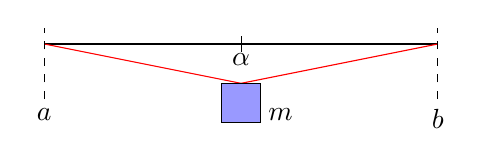
\begin{tikzpicture}
\draw (0,0) -- (5,0);
% parabola
\draw[scale=1,domain=0:2.5,smooth,variable=\x,red] plot ({\x}, {-0.2*\x});
\draw[scale=1,domain=2.5:5,smooth,variable=\x,red] plot ({\x}, {0.2*(\x-5)});

% etiquetas
\draw[dashed] (0,-0.7) -- (0,.2);
\draw (0,-0.7) node[anchor=north] {$a$};
\draw[dashed] (5,-.7) -- (5,.2);
\draw (5,-0.7) node[anchor=north] {$b$};
\draw (2.5,-0.1) -- (2.5,.1);
\draw (2.5,0) node[anchor=north] {$\alpha$};
\draw (3,-0.7) node[anchor=north] {$m$};

% masa
\fill[blue!40!white, draw=black] (2.25,-1) rectangle (2.75,-0.5);
\end{tikzpicture}
\end{center}
La forma bilineal $A$ es la misma que en el anterior modelo:
\[
A(y,y)=\frac{1}{2}\integral{a}{b}{y'(x)^2dx}+\frac{1}{2}\integral{a}{b}{q(x)y(x)^2dx}
\]
y como estamos en $\sobolevcero{1}$, $\integral{a}{b}{y'(x)^2dx}$ es una norma, luego $A$ es coercivo ya que restando el último término (que es positivo) obtenemos:
\[
A(y,y)\geq \frac{1}{2}\integral{a}{b}{y'(x)^2dx} = \frac{1}{2}\norm{u}^2
\] 
La aplicación lineal y continua $\funcion{R}{\sobolevcero{1}}{\R}$, viene dada por $R(y)=-my(\alpha)$, que tiene sentido al elegir el represante continuo porque $\sobolev{1}\subset \mathcal{C}(a,b)$. Por el teorema de Lax-Milgran (\ref{laxmilgran}) y la proposicion \ref{puntocritico}, existe $y\in\sobolevcero{1}$ de forma que
\[
A(y,\phi)=R(\phi) \espacio \forall \phi\in\sobolevcero{1}
\]
Lo que vamos a hacer ahora es calcular o ver qué condiciones verifica la función $y$. Usando la condición de punto crítico:
\begin{equation}
\label{formulageneral}
\integral{a}{b}{y'(x)\phi'(x)dx}+\integral{a}{b}{q(x)y(x)\phi(x)dx}=-m\phi(\alpha)
\end{equation}
Ahora hacemos una distinción de casos con $\phi$ perteneciendo a diferentes clases de Swartz:
\begin{itemize}[-]
\item si $\phi\in\mathcal{D}(a,\alpha)$:
\[
\integral{a}{b}{y'(x)\phi'(x)dx}+\integral{a}{b}{q(x)y(x)\phi(x)dx}=-m\phi(\alpha)=0
\]
ya que $\alpha\notin(a,\alpha) \Rightarrow \phi(\alpha)=0$. Si denotamos $z=y'$, entonces $z\in\sobolev[a,\alpha]{1}\subset\mathcal{C}[a,\alpha]$ (porque la expresión anterior coincide con la definición de derivada débil para $z$).
\item si $\phi\in\mathcal{D}(\alpha,b)$, de igual forma conseguimos que $z\in\sobolevcero[\alpha,b]{1}\subset\mathcal{C}[\alpha,b]$. 
\end{itemize}
Fijaros que ese razonamiento no implica que $z\in\mathcal{C}[a,b]$, ya que el representante continuo usado en $[a,\alpha]$ y $[\alpha,b]$ son distintos. Lo que si implica es que $z\in\mathcal{C}\left([a,\alpha)\cup(\alpha,b]\right)$ y existen los límites laterales de $\alpha$:
\[
z(\alpha^-)=\limite{x}{\alpha^-}{z(x)} \espacio z(\alpha^+)=\limite{x}{\alpha^+}{z(x)}
\]
Además sabesmos que $z'=qy \;\; a.e \; x \in(a,\alpha)\cup(\alpha,b)$. Si volvemos a la fórmula general \eqref{formulageneral}:
\begin{equation}
\label{formulageneral2}
\integral{a}{b}{z(x)\phi'(x)dx}+\integral{a}{b}{q(x)y(x)\phi(x)dx}=-m\phi(\alpha) \espacio \forall\phi\in\sobolevcero{1}
\end{equation}
Ahora queremos desarrollar esa expresión. Tomamos $\phi\in\soportecompacto$, como $z$ no es continua en $\alpha$, la integral del primer término hay que escribirla en dos partes:
\[
\integral{a}{b}{z(x)\phi'(x)dx}=\integral{a}{\alpha}{z(x)\phi'(x)dx}+\integral{\alpha}{b}{z(x)\phi'(x)dx}
\]
Aplicamos derivación por partes a cada término:
\[
\integral{a}{\alpha}{z(x)\phi'(x)dx}=z(x)\phi(x)\Big|_a^\alpha-\integral{a}{\alpha}{z'(x)\phi(x)dx}=z(\alpha^-)\phi(\alpha)-\integral{a}{\alpha}{z'(x)\phi(x)dx}
\]
\[
\integral{\alpha}{b}{z(x)\phi'(x)dx}=z(x)\phi(x)\Big|_\alpha^b-\integral{\alpha}{b}{z'(x)\phi(x)dx}=-z(\alpha^+)\phi(\alpha)-\integral{\alpha}{b}{z'(x)\phi(x)dx}
\]
Combinando los resultados y sustituyendo en \eqref{formulageneral2}:
\[
z(\alpha^-)\phi(\alpha)-z(\alpha^+)\phi(\alpha)-\integral{a}{b}{z'(x)\phi(x)dx}=-\integral{a}{b}{z'(x)\phi(x)dx}-m\phi(\alpha)
\]
Cancelando ámbos términos:
\[
\left(z(\alpha^-)-z(\alpha^+)\right)\phi(\alpha)=-m\phi(\alpha)
\]
Como la función de Swartz esocgido es arbitraria, podemos suponer quevale 1 en $\alpha$. Usando eso y que $z=y'$:
\[
y'(\alpha^-)-y'(\alpha^+)=-m \Rightarrow y'(\alpha^+)-y'(\alpha^-)=m  
\]
Es decir, el cambio de pendiente que se da entre $\alpha^-$ y $\alpha^+$ es igual a $m$, el peso de la masa.

\subsection{Caso abstracto: problema de Sturm-Liouville}
Vamos a generalizar el caso anterior para obtener una ecuación diferencial con varias condiciones. Sea $\funcion{L}{\sobolev{1}}{\R}$ el funcional dado por:
\[
L(y)=\frac{1}{2}\integral{a}{b}{p(x)y'(x)^2dx}+\frac{1}{2}\integral{a}{b}{q(x)y(x)dx}-R(y)
\]
donde $p,q\in\lebesgue{\infty}$ cumpliendo $0<p_0\leq p(x)\leq p_1$, $0<q_0\leq q(x)\leq q_1$. 

La teoría de Lax-Milgran nos dice que:
\[
A(y,\phi)=R(\phi) \Rightarrow \integral{a}{b}{p(x)y'(x)\phi'(x)dx}+\integral{a}{b}{q(x)y(x)\phi(x)dx}=R(\phi)
\]
Y denotando $z=py'$ se verifica $z'=qy-R(\phi)$.

\begin{definition}
Sean $p,q\in\lebesgue{\infty}$ cumpliendo $0<p_0\leq p(x)\leq p_1$, $0<q_0\leq q(x)\leq q_1 \;\; \casipordoquier$. La ecuación de Sturm-Liouville viene dada por la expresión:
\[
(p(x)y'(x))'-q(x)y(x)=R(\phi)
\]
\begin{itemize}
\item Si $y\in\sobolevcero{1}$, consideramos $R\in(\sobolevcero{1})^*$.
\item Si $y\in\sobolev{1}$, consideramos $R\in(\sobolev{1})^*$.
\end{itemize}
\end{definition}
\begin{definition}
Una solución débil de la ecuación de Sturm-Lioville es una función $y$ verificando la expresión anterior.
\begin{itemize}
\item Si $y\in\sobolevcero{1}$, entonces $y(a)=y(b)=0$ (caso Dirichlet).
\item Si $y\in\sobolev{1}$, entonces $y'(a)=y'(b)=0$ (caso Neumann).
\end{itemize}
\end{definition}
\begin{remark}
Si consideramos $R\in(\sobolev{1})^*$, la condición $y'(a)=y'(b)=0$ nos aparece de forma natural al minimizar (visto anteriormente).
\end{remark} 

A partir de ahora nos vamos a centrar en el caso $y\in\sobolev{1}$, $R\in(\sobolev{1})^*$.

\textbf{que vamos a hacer a continuacion?}

\begin{remark}
Recordemos una propiedad del Análisis funcional respecto a duales: (\textbf{DUDOSA})
\begin{center}
\begin{tikzpicture}[node distance=2.5cm, auto]
\node (A) {$\sobolev{1}$};
\node (B) [right of=A] {$\sobolev{1}$};
\node (C) [below of=A] {$(\sobolev{1})^*$};
\node (D) [below of=B] {$(\sobolev{0})^*$};
\draw[->](A) to node {$i$}(B);
\draw[->, dashed](B) to node [] {}(D);
\draw[->, dashed](A) to node [] {}(C);
\draw[->](D) to node [above] {$i^*$}(C);
\end{tikzpicture}
\end{center}
donde $i^*$ es la aplicación traspuesta de $i$. Veámoslo con un ejemplo concreto, supongamos que tenemos $n<m$:
\begin{center}
\begin{tikzpicture}[node distance=2cm, auto]
\node (A) {$\R^n$};
\node (B) [right of=A] {$\R^m$};
\node (C) [below of=A] {$\R^n$};
\node (D) [below of=B] {$\R^m$};
\draw[->](A) to node {$i$}(B);
\draw[->, dashed](B) to node [] {}(D);
\draw[->, dashed](A) to node [] {}(C);
\draw[->](D) to node [above] {$i^*$}(C);
\end{tikzpicture}
\end{center}
donde $i\in\mathcal{M}_{n\times m}$ y $i^*\in\mathcal{M}_{m\times n}$. Lo esperable es que si $i$ es inyectiva, es decir, el rango de $i$ es $n$, entonces la otra matriz también tiene rango $n$, pero eso quiere decir que es sobreyectiva. Es decir, esta dualidad nos pasa aplicaciones inyectivas a aplicaciones sobreyectivas. A nosotros nos interesa ver la inclusión de los espacios "relativamente bien", puesto que el al fin y al cabo el Teorema de Riesz nos dice que todos los espacios de Hilbert son iguales, pero no quiero perder la estructura ni las inclusiones entre ellos.
\end{remark}

\duda{no me queda claro el propósito de esta nota}

Si ahora tomamos $g\in\lebesgue{2}=\sobolev{0}$, podemos definir la función $\funcion{R_g}{\sobolev{1}}{\R}$ por
\[
R_g(y)=\integral{a}{b}{g(x)y(x)dx} 
\]

Aquí dijimos $R_g\in(\sobolev{1})^*=\sobolev{-1}$. Tambíen hablamos de la inclusión
\[
\sobolev{2}\subset\sobolev{1}\subset\sobolev{-1}
\]

\begin{definition}
Dado $\alpha\in(a,b)$, definimos la función $\funcion{\delta_\alpha}{\sobolev{-1}}{\R}$
\[
\delta_\alpha(y)=y(\alpha), \espacio \delta_\alpha\in\sobolev{1}, \;\; \delta_\alpha\notin\sobolev{0}
\]
A $\delta_\alpha$ se le llama $\delta$ de Dirach.
\end{definition}

\duda{no sé que significa lo de abajo}

\[
(py')'-qy=\delta_\alpha
\]
\[
(py')(\alpha^+)-(py')(\alpha^-)=+1
\]

\duda{duda generalizada del caso Dirichlet caso Neumann, según he ententido: antes de esta nota hemos definido el problema de Sturm-Liouville, y ahora consideramos dos casos diferentes (dirichlet y neumann) según donde tomemos la y???}

\subsection*{Problema de Sturm-Liouville}
Vamos a escribir formalmente el problema de Sturm-Liouville. Para ello, tomamos el siguiente funcional: 
\[
L(y)=\frac{1}{2}\integral{a}{b}{p(x)y'(x)^2dx}+\frac{1}{2}\integral{a}{b}{q(x)y(x)^2dx}-R(y)
\]
con $p,q\in\lebesgue{\infty}$, $0<p_0\leq p(x)\leq p_1 \; \casipordoquier$. 

Existen dos casos distintos de este problema, dependiendo de donde consideremos la función $y$, es decir, dependiendo de donde queramos minimizar:
\begin{definition}[Caso Dirichlet]
Sea $\funcion{L}{\sobolevcero{1}}{\R}$ y establecemos las siguientes condiciones:
\begin{enumerate}[(a)]
\item $y\in\sobolevcero{1}: \; y(a)=y(b)=0$
\item $0\leq q(x)\leq q_1 \; \casipordoquier$
\item $R\in(\sobolevcero{1})^*$
\end{enumerate}
\end{definition}
\begin{definition}[Caso Neumann]
Sea $\funcion{L}{\sobolev{1}}{\R}$ y establecemos las siguientes condiciones:
\begin{enumerate}[(a)]
\item $y\in\sobolev{1}: \; y'(a)=y'(b)=0$
\item $0<q_0\leq q(x)\leq q_1 \; \casipordoquier$
\item $R\in(\sobolev{1})^*=\sobolev{-1}$
\end{enumerate}
\end{definition}
\begin{remark}
A partir de ahora, cuando pongamos \circled{D} o \circled{N}, haremos referencia a las condiciones del caso Dirichlet o Neumann respectivamente.
\end{remark}
\duda{se ha hablado en varias ocasiones sobre las condiciones que se imponen, pero no me acaban de quedar clara porque imponemos cada una, podría añadir un breve comentario sobre cada una de ellas?}
En cualquiera de los dos casos, el teorema de Lax-Milgran (\ref{laxmilgran}) nos confirma la existencia de solución y nos da la condición de punto crítico (dependiente del caso en el que estemos):
\begin{equation}
\label{criticoliouville}
A(y,\phi)=R(\phi) \Rightarrow \integral{a}{b}{p(x)y'(x)\phi'(x)dx}+\integral{a}{b}{q(x)y(x)\phi(x)dx}=R(\phi)
\end{equation}
\begin{itemize}
\item Para toda $\phi$ en $\sobolevcero{1}$, en el caso Dirichlet.
\item Para toda $\phi$ en $\sobolev{1}$, en el caso Neumann.
\end{itemize}
Formalmente, si llamo $z(x)=p(x)y'(x)$, la expresión \eqref{criticoliouville} me diría que $z'(x)=q(x)y(x)-R$. Fijaros que $R$ no es una función, sino un elemento del dual y que lo único que sabemos es que $y$ está en $\sobolev{1}$, luego no tenemos información sobre $z$. 

Esa ecuación se escribe formalmente como:
\[
(p(x)y'(x))'-q(x)y(x)=R \text{ (Problema de Sturm-Liouville) }
\]
junto con una condición \circled{D} o \circled{N}. 

Si ahora a $R$ la denotamos por $f$, la ecuación quedaría:
\begin{equation}
\label{problemaliouville2}
(p(x)y'(x))'-q(x)y(x)=f(x)
\end{equation}
Fijaros que hemos añadido $(x)$ al lado de $f$, pero realmente $f$ no es una funcion, sino que es un elemento de $(\sobolevcero{1})^*$ (caso \circled{D}) o de $\sobolev{1}$ (caso \circled{N}). Pero recordad que $\lebesgue{2}=\sobolev{0}\hookrightarrow\sobolev{-1}$, ¿cómo hacemos esa inclusión? Con $R_g$, definida anteriormente:
\[
f\mapsto R_f(y)=\integral{a}{b}{f(x)y(x)dx}
\]
\duda{a parte, $R_f(y)\in\R$, cómo va a estar en $\sobolev{1}$ si eso es un espacio de funciones?}
\duda{aqui usamos $R_f$, definido en la clase anterior pero no me queda claro por qué}

\begin{itemize}
\item Si $f\in\sobolev{0} \Rightarrow p(x)y'(x)\in\sobolev{1}$ y tenemos la siguiente ecuación diferencial
\[
(p(x)y'(x))'-q(x)y(x)=f(x)
\]
más la condición \circled{N}, donde esas derivadas sí son débiles.
\item Si $f=\displaystyle\sum_{i=1}^kc_i\delta_{\alpha_i}$ donde $a<\alpha_1,...,\alpha_k<b$ y $c_1,...,c_k\in\R$.

Denotando $z(x)=p(x)y'(x)$, tenemos que $z$ verifica la expresión \eqref{problemaliouville2}:
\begin{equation}
\label{intentandoentenderesto}
\integral{a}{b}{z(x)\phi'(x)dx}+\integral{a}{b}{q(x)y(x)\phi(x)dx}=\sum_{i=0}^kc_i\delta_{\alpha_i}=\sum_{i=0}^kc_i\phi(\alpha_i)
\end{equation}
para toda $\phi$ en $\sobolevcero{1}$ si \circled{D} o en $\sobolev{1}$ si \circled{N}.

Si ahora tomamos $\phi\in\mathcal{D}(a,b)$ de forma que en cada intervalo $(\alpha_{i-1},\alpha_{i+1})$ se cumpla:
\begin{figure}[H]
   \center
  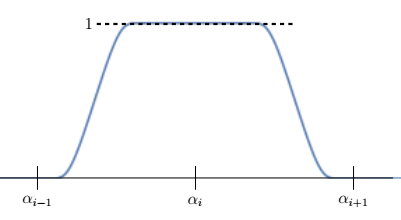
\includegraphics[scale=0.6]{img/flatproof.png}
\end{figure}
y consideramos $z$ como la unión de los representantes continuos en cada intervalo, es decir,
$z\in\mathcal{C}\left([a,\alpha_1)\cup...\cup(\alpha_k,b]\right)$, tenemos que $z'(x)=q(x)y(x) \; \casipordoquier$. Aplicando la expresión \eqref{intentandoentenderesto} a cada intervalo $((\alpha_{i-1},\alpha_{i+1}))$ nos queda:
\begin{equation}
\label{comparando}
\integral{\alpha_{i-1}}{\alpha_{i+1}}{z(x)\phi'(x)dx}+\integral{\alpha_{i-1}}{\alpha_{i+1}}{z'(x)\phi(x)dx}=c_i\phi(\alpha_i)
\end{equation}
Si separamos la integral del primer término en dos, en los intervalos $(\alpha_{i-1},\alpha_{i})$ y $(\alpha_{i},\alpha_{i+1})$ y aplicamos la regla de la cadena:
\[
\integral{\alpha_{i-1}}{\alpha_{i}}{z(x)\phi'(x)dx}=z(x)\phi(x)\Big|_{\alpha_{i-1}}^{\alpha_{i}}-\integral{\alpha_{i-1}}{\alpha_{i}}{z'(x)\phi(x)dx}=z(\alpha_{i}^-)-\integral{\alpha_{i-1}}{\alpha_{i}}{q(x)y(x)\phi(x)dx}
\]
\[
\integral{\alpha_{i}}{\alpha_{i+1}}{z(x)\phi'(x)dx}=z(x)\phi(x)\Big|_{\alpha_{i}}^{\alpha_{i+1}}-\integral{\alpha_{i}}{\alpha_{i+1}}{z'(x)\phi(x)dx}=-z(\alpha_{i}^+)-\integral{\alpha_{i}}{\alpha_{i+1}}{q(x)y(x)\phi(x)dx}
\]
Sumando ahora esos dos resultados y volviendo a combinar las integrales:
\[
\integral{\alpha_{i-1}}{\alpha_{i+1}}{z(x)\phi'(x)dx}=z(\alpha_{i}^-)-z(\alpha_{i}^+)-\integral{\alpha_{i-1}}{\alpha_{i+1}}{q(x)y(x)\phi(x)dx} \Rightarrow
\]
\[
\integral{\alpha_{i-1}}{\alpha_{i+1}}{z(x)\phi'(x)dx}-\integral{\alpha_{i-1}}{\alpha_{i+1}}{q(x)y(x)\phi(x)dx}=z(\alpha_{i}^-)-z(\alpha_{i}^+)
\]
Si nos fijamos, a la izquierda tenemos lo mismo que en la expresión \eqref{comparando}, luego igualando:
\[
z(\alpha_{i}^-)-z(\alpha_{i}^+)=c_i\phi(\alpha_i)=c_i \Rightarrow
\]
\[
z(\alpha_{i}^+)-z(\alpha_{i}^-)=-c_i
\]
\duda{que hemos conseguido con esto?}
\end{itemize}
